\frame{
  \frametitle{Introduction}

  \begin{itemize}
    \item Billiard ball bouncing in a square
    \item Assume no gravity or friction
    \item Examine sequence of sides
  \end{itemize}
}

\subsection{Examples}

\frame{
  \frametitle{Example}

  \begin{example}
    Examine the sequence: `abab`
  \end{example}

  \begin{figure}
    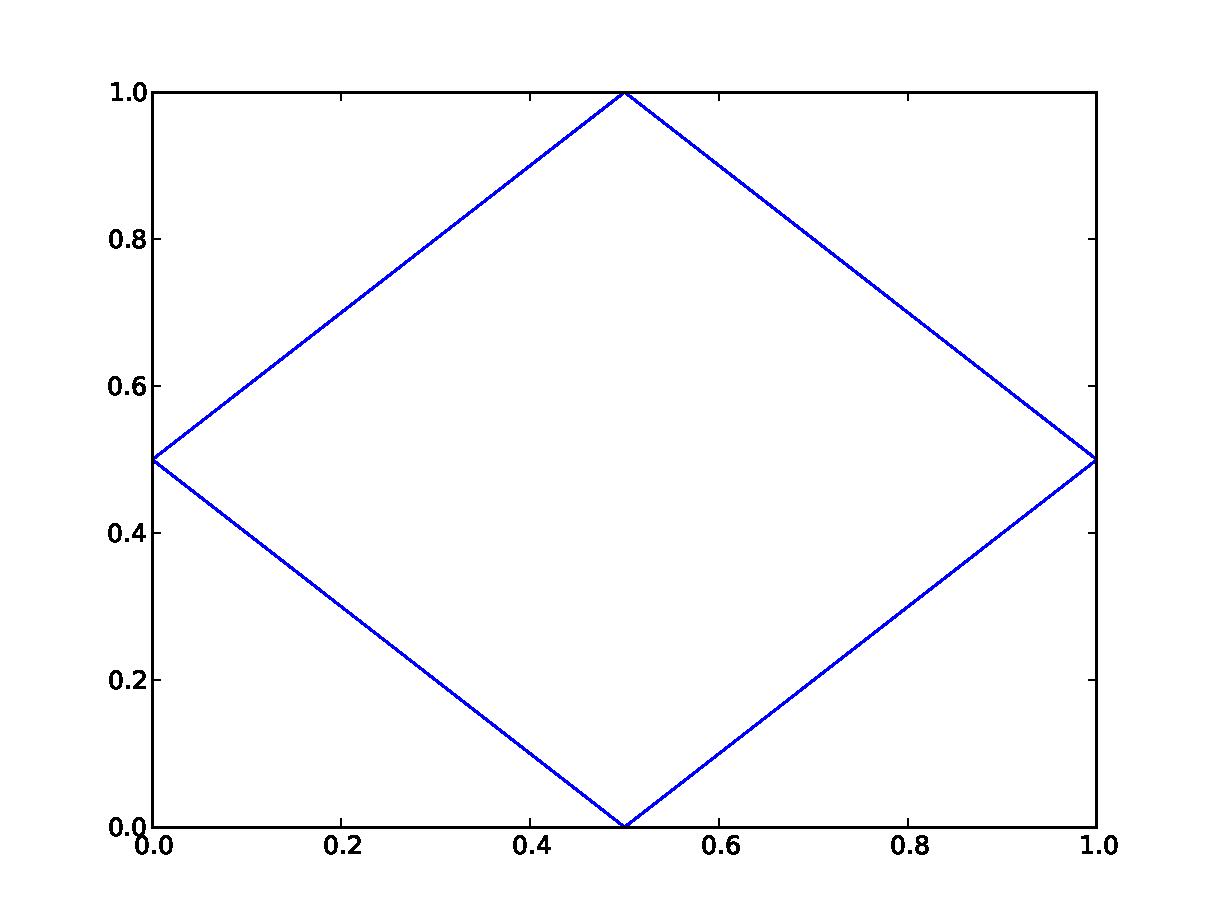
\includegraphics[width=3in]{figures/abab.pdf}
  \end{figure}
}

\frame{
  \frametitle{Another Example}

  \begin{example}
    Examine the sequence: `aaabaaab`
  \end{example}

  \begin{figure}
    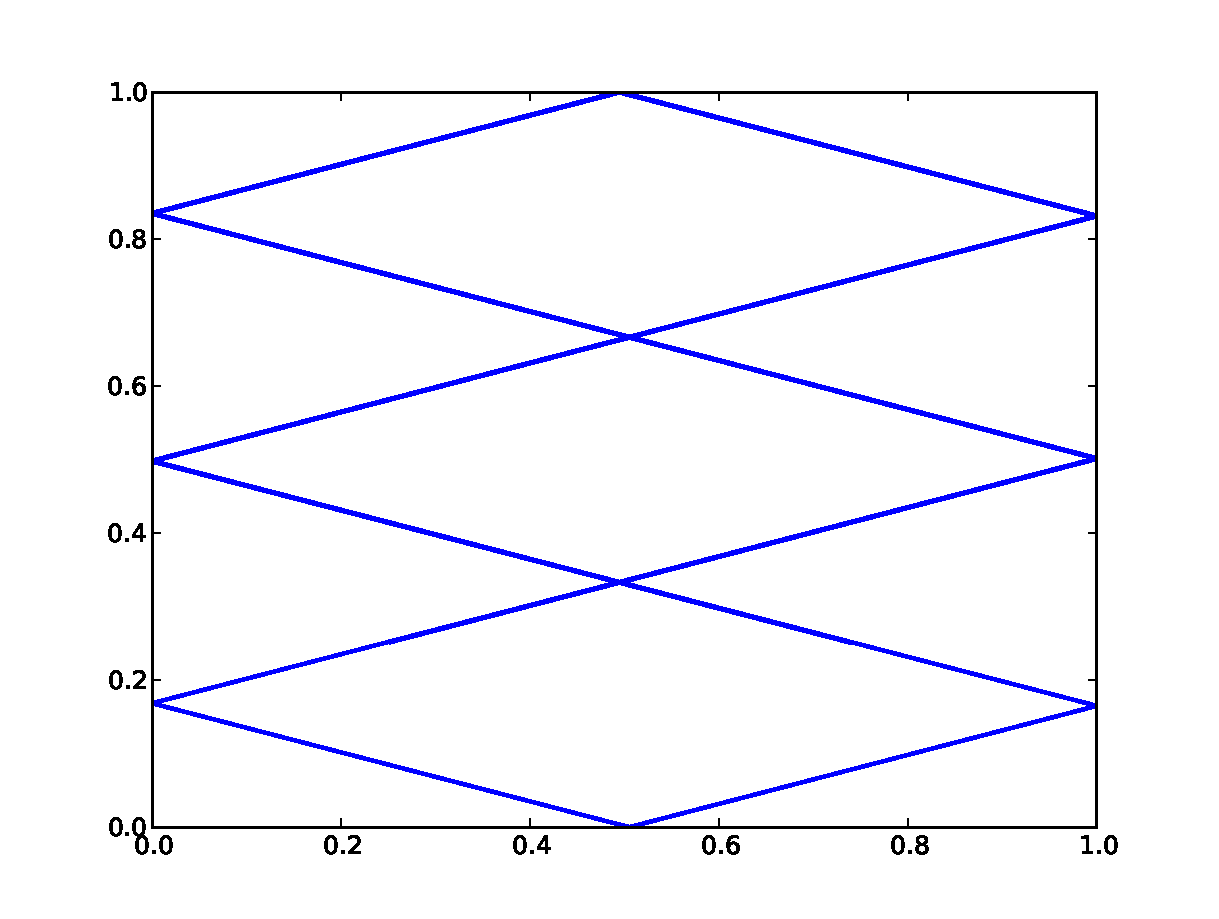
\includegraphics[width=3in]{figures/aaabaaab.pdf}
  \end{figure}
}

\subsection{Outline}

\frame{
  \frametitle{Presentation Outline}
  \tableofcontents
}

\frame{
  \frametitle{Notation}

  \begin{definition}
    A table $T$ is the unit square in $\mathrm{R}^2$. A particle $p \in T$ begins at position $\bar{x}_0 \in T$ with velocity $\bar{v}$. When the particle reaches an edge of the table, velocity is reflected about the line perpendicular to the table's edge.
  \end{definition}

  \begin{figure}
    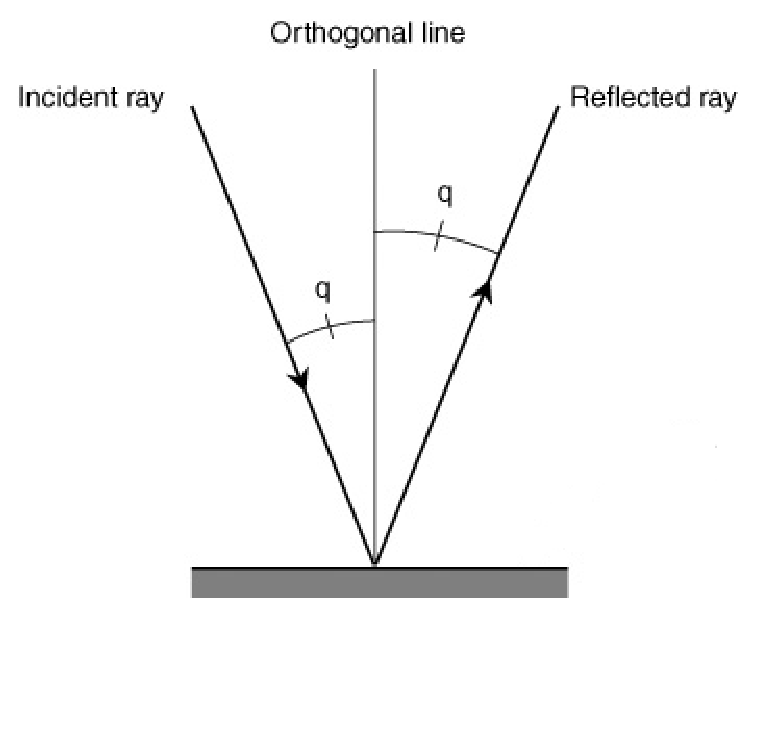
\includegraphics{figures/particle_collision.eps}
  \end{figure}
}

\frame{
  \frametitle{Notation}
  \begin{definition}
    Sequence
  \end{definition}
}

\subsection{Problem Statement and Notation}

\frame{
  \frametitle{Problem Statement}

  Problem: What properties of s
}

